% Provenance (never printed): see sources/outline_sources.md (Year 2: taphonomy; index fossils;
% facies and fossils as environment markers; reconstructing a palaeoenvironment from a map and a
% section). Taphonomy after Loron (2024); live, dead and fossil assemblages after Tyler and
% Kowalewski (2025); Lagerstaetten after Gaines and others (2024), Mussini and Butterfield
% (2025), Vannier and others (2018), Gerschermann and others (2021) and Rauhut and others
% (2018); zone durations after Al-Suwaidi and others (2022); ichnofacies after Buatois and others
% (2020) and Paz and others (2023); stenohaline groups after McGairy and others (2021) and Saleh
% and others (2022). The Varden column from figdata/shared/region.py; porosities and rates from
% figdata/bachelor-2/palaeoenv.py; exercise and problem values in the Book 4 scratch calculator
% calc/ch20.py. The fossil content given to the Varden units is invented, like the region.
\chapter{化石与古环境}\label{ch:b2:palaeoenvironments}

在一块灰色砂岩板上，留有三条线索：三叶虫在泥中拖行留下的痕迹、
水流留下的波痕，以及一个被蠕虫挖掘后又遗弃的洞穴。这三者都不是完整的动物，
但合在一起说明，这片山坡曾是海底，海水浅到足以让波浪搅动海底，
水又咸到三叶虫能在其中生活。化石是过去生命的遗体和遗迹，地质学家
从两个方面解读它们：把它们当作给岩石定年的“时钟”，也当作岩石形成地点的“见证”。本章追随一个生物从死亡到收藏者抽屉的历程，
打开那些连软体也能保存的罕见沉积物，然后
用数字读出一片已消失的海的环境，
其依据来自瓦尔登丘陵的覆盖岩层。
% ledger: usgs:fossil-record-bulk, loron24:taphonomy

\begin{recall}
\textbf{来自中小学分册}：化石、外模、内模和\omterm{def:b2:palaeoenvironments:fossil-kinds}{遗迹化石}；埋藏与矿物如何使贝壳变成石头；
化石随时间的更替。\textbf{来自本科一年级分册}：
沉积相与沉积环境、浊积岩、礁和鲕粒；生物带、标准化石
与首现面；压实、去压实、阿西定律与岩层的固体厚度；
胶结物；可容纳空间。\textbf{来自前面各章}：\omterm{def:b2:phanerozoic-earth:transgression}{海侵}与\omterm{def:b2:phanerozoic-earth:transgression}{海退}，
长期海平面与\omterm{def:b2:phanerozoic-earth:oae}{大洋缺氧事件}（见\cref{ch:b2:phanerozoic-earth}）。物种如何演化，以及动植物如何分类，
则属于生物学分册的内容。
\end{recall}

\section{从死亡到化石}\label{sec:b2:palaeoenvironments:taphonomy}

大多数生物什么也不会留下。细菌与食腐动物会在数天或数年内吞食软组织，
水流会打碎并冲散硬组织，土壤与孔隙水中的酸则溶解残余的部分。
化石是熬过上述所有作用而留存下来的东西，
还须再经受埋藏、加热以及包裹它的岩石的隆升。

\begin{definition}[埋藏学；保存潜力]\label{def:b2:palaeoenvironments:taphonomy}
\emph{埋藏学}\index{埋藏学}研究生物遗体
从死亡到被发现为化石的全过程中所发生的事情：腐烂、食腐、搬运、埋藏，以及成岩作用引起的化学变化。
生物体或其某一部分的\emph{保存潜力}\index{保存潜力}，
是指它经历上述各阶段
并留存于岩石中的概率。
\end{definition}
% ledger: loron24:taphonomy

每个阶段都会移除某些东西、增添某些东西，或改变某些东西。腐烂与食腐移除软组织；
孔隙水中的矿物充填骨骼的孔隙，或替换贝壳中的文石，
增添了动物原本没有的物质；加热则改变残留的有机分子。
洛龙把所有这些死后变化分为三类：增益、损失与改变，
并将它们写成一个方程，用以表示生物与其化石之间任一可测量特征的变化。
下图展示了各阶段及其所带走的东西。
% ledger: loron24:taphonomy

\begin{omfigure}
\centering
\begin{tikzpicture}[font=\scriptsize, x=1cm, y=1cm,
  stage/.style={draw=black!60, fill=omSea!12, rounded corners=2pt, align=center,
    text width=2.05cm, minimum height=1.25cm, inner sep=2pt},
  loss/.style={align=center, text width=2.05cm, text=omThm!80!black}]
\node[stage] (a) at (0,0) {\textbf{死亡}\\一个活的 \\群落};
\node[stage] (b) at (2.75,0) {\textbf{腐烂与}\\\textbf{食腐}\\位于海底};
\node[stage] (c) at (5.5,0) {\textbf{搬运}\\水流分选 \\并打碎};
\node[stage] (d) at (8.25,0) {\textbf{埋藏}\\位于 \\活动层之下};
\node[stage] (e) at (11,0) {\textbf{成岩作用}\\压实、\\置换};
\node[stage] (f) at (13.75,0) {\textbf{折返}\\与 \\采集};
\foreach \u/\v in {a/b, b/c, c/d, d/e, e/f} {\draw[-{Stealth[length=2mm]}, black!70] (\u) -- (\v);}
\node[loss, anchor=north] at (2.75,-0.8) {软组织丢失；\\骨骼散架};
\node[loss, anchor=north] at (5.5,-0.8) {轻质部分被带走，\\贝壳破碎};
\node[loss, anchor=north] at (8.25,-0.8) {埋藏缓慢：\\给损失留下更多时间};
\node[loss, anchor=north] at (11,-0.8) {文石溶解，\\增添矿物};
\node[loss, anchor=north] at (13.75,-0.8) {被侵蚀殆尽，\\或从未被发现};
\end{tikzpicture}
\par\smallskip{\small 从活的群落到标本收藏的埋藏路径，以及
各阶段所移除或改变的内容。埋藏是转折点：埋藏之前，遗体暴露于
一切损失之中；埋藏之后，只有成岩作用和侵蚀作用对其起作用。}
\end{omfigure}
% ledger: loron24:taphonomy

中小学分册把任何保存在岩石中的过去生命的遗体或遗迹都称为化石。
两类化石在岩石中的表现差异很大，理应各有专门的名称。

\begin{definition}[实体化石；遗迹化石]\label{def:b2:palaeoenvironments:fossil-kinds}
\emph{实体化石}\index{实体化石}是生物身体的一部分，或该部分的外模或内模，
例如贝壳、骨、牙齿、叶，在罕见的沉积物中还可以是软组织。
\emph{遗迹化石}\index{遗迹化石}是生物在沉积物或岩石中或其表面
活动时形成的构造：足迹、爬迹、洞穴、钻孔与取食痕迹。
\end{definition}

\omterm{def:b2:palaeoenvironments:fossil-kinds}{遗迹化石}是其所挖掘的沉积物的一部分：水流若将其搬走，它便会被毁坏。
因此，它记录了制造者生活之处的条件，而
易沿海底滚动的贝壳则不一定能做到这一点。\omterm{def:b2:palaeoenvironments:fossil-kinds}{遗迹化石}的命名与生物相同，
同样有属和种，但这一名称描述的是构造，而非动物本身：
同一个洞穴可以由多种动物挖掘而成，一种动物也可以留下多种遗迹。

\subsection*{埋藏与毁坏之争}

埋藏与毁坏之争可以用一个简单的模型来描述。躺在海底的遗体
以恒定速率 $k$ 遭受毁坏，此即单位时间内它们被吞食、
破碎或溶解的概率；一旦被厚度为 $h$ 的沉积物覆盖，它们便安全；
沉积物则以速率 $s$ 堆积。

\begin{proposition}[埋藏先于毁坏]\label{prop:b2:palaeoenvironments:burial}
在上述假设下，某一遗体抵达安全状态的概率为
\[
  P = e^{-kh/s}.
\]
它只通过埋藏所需时间 $h/s$ 与
海底平均存活时间 $1/k$ 之比依赖于这三个量。
\end{proposition}

\begin{proof}
遗体需要时间 $T = h/s$ 才能被厚度为 $h$ 的沉积物覆盖。若破坏速率为常数
$k$，则 $p(t)$ 为存活至时刻 $t$ 的概率，满足 $p' = -kp$，$p(0) =
1$，于是 $p(t) = e^{-kt}$；取 $t = T$ 时，即为 $e^{-kh/s}$。
\end{proof}

\begin{example}[平静海底上的一枚贝壳]\label{ex:b2:palaeoenvironments:shell}
设一枚贝壳在海底平均存活 20 年，即 $k = \qty{0.05}{\text{年}^{-1}}$，
且在 $h = \qty{0.1}{m}$ 厚的泥下即为安全。当 $s = \qty{1}{mm.\text{年}^{-1}}$ 时，埋藏所需时间为 100
年，$P = e^{-5} = 0.0067$：不到百分之一的贝壳能够存活。当
\qty{1}{cm.\text{年}^{-1}} 时，$P = e^{-0.5} = 0.61$。一场风暴在一天之内倾倒下 \qty{0.3}{m} 的沙，
将海底的一切瞬间掩埋，此时 $P$ 接近 1。数值是假设的，但其中的道理
并非假设：化石富集于沉积物迅速到达之处，或突然成层之处。
\end{example}

该模型也说明了化石记录为何存在偏差。一种软体蠕虫，其在海底的平均存活时间
以天计而非以十年计，其 $k$ 值是厚壳的数百倍，
因而存活概率呈指数级地变小。化石记录的主体由带壳动物
和微观遗骸构成。泰勒与科瓦莱夫斯基检验了一个群落在
进入岩石的途中损失多少。在一片沿海海底的 51 个站点，他们统计到 135 种活的
无脊椎动物，海底遗留的壳与骨骼中有 150 个物种，另有 112 种
也有化石记录。死亡者多于活体，是因为海底的贝壳积累了多年，
来自已不再生活于此处的动物。食碎屑者与肉食性动物多为
软体，最不易被保存；但现生群落的主要生态类群
在\omterm{def:b2:palaeoenvironments:assemblages}{死亡组合}中全部被重新找到。
% ledger: usgs:fossil-record-bulk, tyler25:live-dead, tyler25:soft-bodied

\section{异常保存的窗口}\label{sec:b2:palaeoenvironments:lagerstatten}

\begin{definition}[化石库]\label{def:b2:palaeoenvironments:lagerstatte}
\emph{化石库}\index{化石库}（复数形式为 Lagerstätten）是一种沉积体，它
保存的化石质量极高，尤其是软质、未经生物矿化的组织，这些组织在
别处几乎都会被腐烂破坏。这类沉积体也称为 Konservat-Lagerstätte。
\end{definition}
% ledger: gaines24:konservat

\omterm{def:b2:palaeoenvironments:lagerstatte}{化石库}罕见，但人们对软体动物的大部分认识来自这些地方，
而动物的第一次大辐射（发生于寒武纪）也最好借助它们来理解。
% ledger: gaines24:konservat

\subsection*{伯吉斯页岩}

1909 年，查尔斯·沃尔科特在其野外笔记中素描了一种小型节肢动物，它是他在伯吉斯
页岩（位于不列颠哥伦比亚）中发现的。此后他在同一层段中采集了数百件
\emph{Waptia} 标本，取自厚约 \qty{2}{m} 的单一层段，即 Phyllopod
层；其现代描述依据藏于两家博物馆的 1800 多件标本。伯吉斯
页岩形成于约 5.08 亿年前，当时沉积于较深水域，面向一处陡峭的海底
陡崖。其化石包括无壳动物，以扁平碳膜的形式保存，
常为完整个体。这种保存与埋藏于贫氧泥中密切相关，其中动物不曾
掘穴，水流也不曾改造沉积：上图中的损失在此一举得以阻止。
% ledger: vannier18:waptia, mussini25:burgess

\begin{omfigure}
\centering
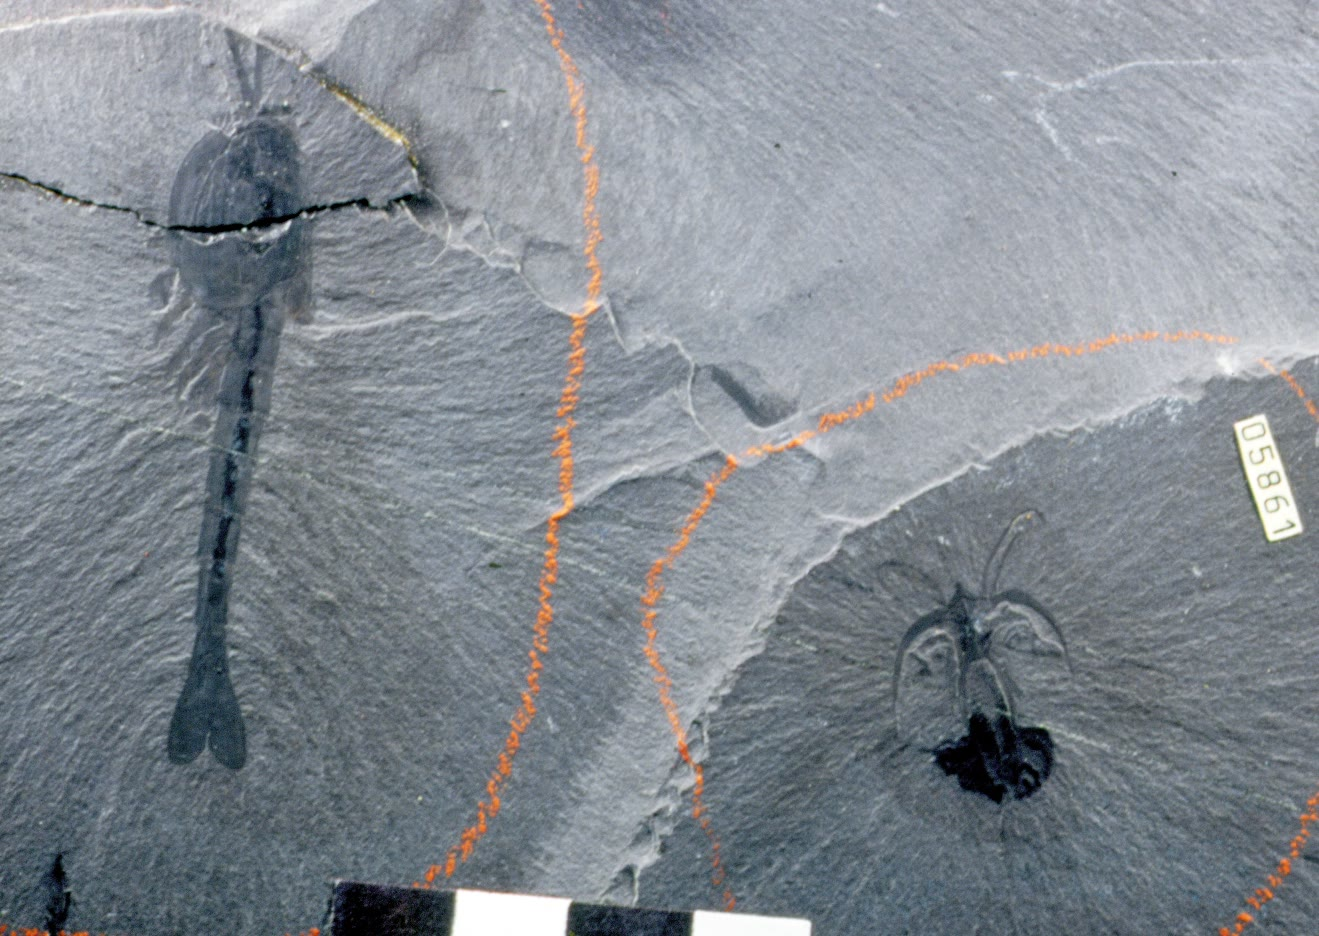
\includegraphics[width=0.72\linewidth]{images/book4/b2-20-burgess-waptia-marrella.jpg}
\par\smallskip{\small 伯吉斯页岩中的两种节肢动物，以暗色碳膜形式保存：
\emph{Waptia}（左）与 \emph{Marrella}（右）。（照片：James
St.~John, CC~BY~2.0，经维基共享资源。）}
\end{omfigure}
% ledger: mussini25:burgess

\subsection*{索伦霍芬}

巴伐利亚的索伦霍芬与艾希施泰特的细粒石灰岩，沉积于泻湖之中，
时间为提通阶早期（侏罗纪最后一个阶，始于 \qty{149.2}{Ma} 前），此处是
十二件 \emph{Archaeopteryx} 标本、众多翼龙以及鱼类的模式产地，其中鱼类的
软组织乃至颜色图案都得以保存。该地化石罕见，但其
保存状况极为出色。人们提出了数种条件，或许共同起作用：
底水盐度约为海水的三倍，或极度碱性，它们都会减缓细菌
分解；细菌席封住了尸体；无氧底水使
食腐动物远离；风暴搅起石灰泥并迅速掩埋尸体。这些因素中的每一个
都会延长存活时间 $1/k$，或缩短埋藏时间 $h/s$。
% ledger: gerschermann21:solnhofen, rauhut18:archaeopteryx, ics4:jurassic-stages

\begin{omfigure}
\centering
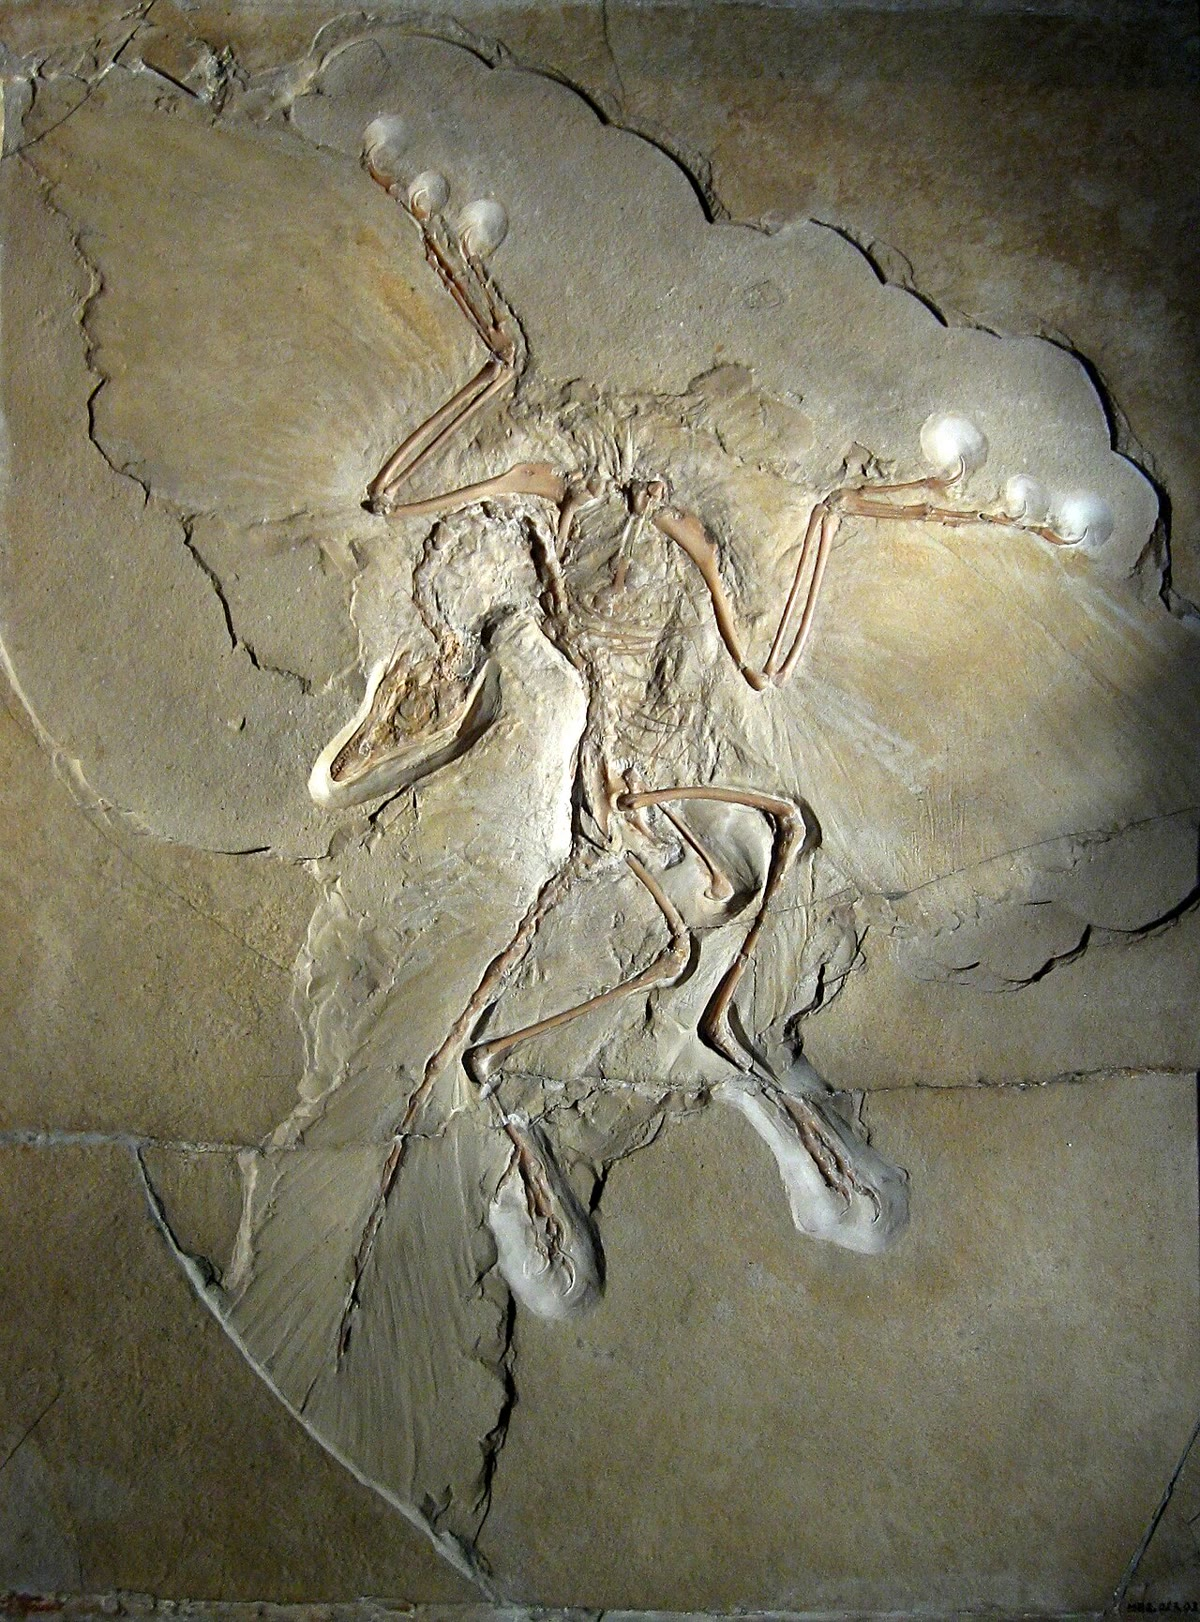
\includegraphics[width=0.5\linewidth]{images/book4/b2-20-archaeopteryx-berlin.jpg}
\par\smallskip{\small 柏林的 \emph{Archaeopteryx} 标本，产自索伦霍芬
石灰岩：翅膀与尾部的骨骼及羽毛印痕。（照片：H.~Raab, CC~BY-SA~3.0，
经维基共享资源。）}
\end{omfigure}
% ledger: rauhut18:archaeopteryx, gerschermann21:solnhofen

\subsection*{化石作为时钟}

本科一年级分册中建立了生物带的概念，即由其化石界定的一套地层，以及
用以识别它的标准化石。这些化石能构成多精细的时钟？一个侏罗纪菊石带可持续
约一百万年：最早的托阿尔阶菊石带，以铀–铅法测定阿根廷
火山灰层的年龄，跨度为 183.73 至 \qty{182.77}{Ma}。带又分为层位，侏罗纪晚期
的一个菊石层位平均持续 \qty{165}{ka}。\emph{Archaeopteryx} 的全部骨骼
均产自同一个含五个层位的带，因此该鸟类的已知时间跨度
约为 70 万至 100 万年。化石本身只能给出先后次序；以年计的年代来自
经铀和铅测定的火山灰层，以及沉积旋回。同一批火山灰层将托阿尔阶底界定为 $183.73$，其不确定度为
$+0.35$ 与 \qty{-0.50}{Ma}，而国际年代表给出 \qty{184.2}{Ma}。
% ledger: alsuwaidi22:toarcian, rauhut18:archaeopteryx, ics4:jurassic-stages

\section{化石作为环境的见证}\label{sec:b2:palaeoenvironments:environment}

要从化石中读出环境，地质学家假定生物生活在其现生
近亲所在之处，并假定今日作用于沉积物的过程，当时亦以同样方式起作用。

\begin{definition}[现实主义原理]\label{def:b2:palaeoenvironments:actualism}
\emph{现实主义原理}\index{现实主义原理}是一种解释过去地质记录的方法，即借助
今日可观察到的过程，以及生物与其环境之间的关系。
\end{definition}

1830 年，赖尔为其 \emph{Principles of Geology} 第一卷加的副标题是：“
试图借助现今仍在起作用的原因，解释地球表面以往的变化
”。该方法有其局限。许多类群已经灭绝，其生活方式必须
由其形态及周围沉积物推断；过去的某一环境，或许
今日并无确切的对应物。
% ledger: lyell1830:title

\begin{definition}[古环境]\label{def:b2:palaeoenvironments:palaeoenvironment}
一个\emph{古环境}\index{古环境}是指岩石形成之地点与时代所占优势的物理、化学与生物条件之总和：
所处的背景、水的深度与能量、
水的盐度、温度与氧含量、底面的性质，
以及其上的生物。
\end{definition}

\subsection*{化石生活在何处？}

首先要问的是，化石是否就生活在它们所在的位置。

\begin{definition}[生活组合与死亡组合；原地化石与外来化石]\label{def:b2:palaeoenvironments:assemblages}
\emph{生活组合}\index{生活组合}是指一群曾共同生活的生物化石，
其保存位置与生活位置一致；\emph{死亡组合}\index{死亡组合}是指死后被聚集在一起的遗骸群，
其中可能混杂来自不同地点、不同时代的生物。
若化石保存于生物生活的地点，则称其为\emph{原地}\index{原地化石}的；
而若化石在埋藏之前
已被搬运至别处，则称其为\emph{外来}\index{外来化石}的。
\end{definition}

搬运的线索如下。壳体仍然闭合，珊瑚或穴居双壳类保持其生长位置，
脆弱的棘刺完好无损，种群的各个年龄段均有保存：这些化石很可能是\omterm{def:b2:alpine-orogen:nappes}{原地的}。
单个壳瓣按大小分选，磨损与破碎的碎片，
或壳体集中于递变层底部：则说明它们曾被搬运。上图中海岸底面的那种贝壳\omterm{def:b2:palaeoenvironments:assemblages}{死亡组合}，
仍保留了群落的大部分成员，但它将许多年的生物汇集于同一层中，
其化石在时间上被平均化了。
% ledger: tyler25:live-dead

\subsection*{盐度与氧含量}

有些动物只能耐受外海的盐度，称为窄盐性的。棘皮动物、
头足类、珊瑚，以及古生代的三叶虫，是典型的窄盐性类群；
它们的出现说明海水正常，而其在丰富动物群中的缺席则可能说明相反的情况。
越南一处志留纪河口的沉积物中保存有植物碎屑、鱼骨、双壳类、腹足类
与介形虫，却没有上述任何一类。棘皮动物也不见于澄江生物群，
这一约 5.18 亿年前的\omterm{def:b2:palaeoenvironments:lagerstatte}{化石库}，
尽管它们见于寒武纪的外海\omterm{def:b2:palaeoenvironments:lagerstatte}{化石库}中：澄江动物生活于三角洲附近，淡水使盐度发生波动。
% ledger: mcgairy21:stenohaline, saleh22:echinoderms, saleh22:age

氧含量通过穴居生物留下印记。底层水体含氧时，动物会搅动沉积物，
破坏其细微的纹层；底层水体无氧时，纹层得以保存，不见潜穴，
并形成黄铁矿，如\cref{ch:b2:phanerozoic-earth}中\omterm{def:b2:phanerozoic-earth:oae}{大洋缺氧事件}的黑色页岩。
同样缺乏穴居生物，
使伯吉斯页岩的动物尸体得以保存。
% ledger: mussini25:burgess

\subsection*{遗迹相}

\omterm{def:b2:palaeoenvironments:fossil-kinds}{遗迹化石}是底面最好的见证者，因为它们并未被移动。造迹生物
会对水的能量、底面的坚硬程度、食物与氧含量作出反应，
显生宙中同一组遗迹组合反复出现。

\begin{definition}[遗迹相]\label{def:b2:palaeoenvironments:ichnofacies}
\emph{遗迹相}\index{遗迹相}是指反复出现的\omterm{def:b2:palaeoenvironments:fossil-kinds}{遗迹化石}组合，
它反映一组环境条件，并以某一特征性遗迹命名。
\end{definition}

沿海相剖面，从海岸到深盆，依次出现四种海相\omterm{def:b2:palaeoenvironments:ichnofacies}{遗迹相}（见下图）。
\emph{Skolithos} \omterm{def:b2:palaeoenvironments:ichnofacies}{遗迹相}以悬浮摄食者的直立、圆柱形或 U 形居住潜穴为主，
水平遗迹较少，是前滨与临滨的典型\omterm{def:b2:palaeoenvironments:ichnofacies}{遗迹相}。
\emph{Cruziana} \omterm{def:b2:palaeoenvironments:ichnofacies}{遗迹相}以沉积物食者的潜穴为主，
并伴有食草者、肉食者与悬浮摄食者的遗迹，是外陆架的典型\omterm{def:b2:palaeoenvironments:ichnofacies}{遗迹相}：
即正常天气浪基面与风暴浪基面之间的底面，
前者是普通波浪搅动沉积物的深度上限，后者仅风暴浪能够到达。
\emph{Zoophycos} \omterm{def:b2:palaeoenvironments:ichnofacies}{遗迹相}以一种沿中心轴、以螺旋片状改造沉积物的潜穴命名，
是风暴浪基面以下陆架与陆坡的典型\omterm{def:b2:palaeoenvironments:ichnofacies}{遗迹相}。\emph{Nereites} \omterm{def:b2:palaeoenvironments:ichnofacies}{遗迹相}以规则的曲折、螺旋与网状潜穴为特征，
这些潜穴被解读为觅食者稀少的动物所设的陷阱与“花园”，
是陆架边缘以外深海的典型\omterm{def:b2:palaeoenvironments:ichnofacies}{遗迹相}。在半咸水海湾与河口中，
通常只见由少数物种构成的 Cruziana \omterm{def:b2:palaeoenvironments:ichnofacies}{遗迹相}。
% ledger: buatois20:ichnofacies, miguez21:ichnofacies, zhang15:zoophycos, buatois25:graphoglyptids, paz23:nereites

\begin{omfigure}
\centering
\begin{tikzpicture}[font=\scriptsize, x=1cm, y=1cm]
% sea and floor (schematic, not to scale)
\fill[omSea!20] (0.6,0) -- (14,0) -- (14,-3.6) -- (11.2,-3.6) -- (9.6,-1.9) -- (6.2,-1.5)
  -- (3.2,-0.9) -- (1.2,-0.15) -- cycle;
\fill[omLithSand!45] (0,0.25) -- (0.6,0) -- (1.2,-0.15) -- (3.2,-0.9) -- (6.2,-1.5)
  -- (9.6,-1.9) -- (11.2,-3.6) -- (14,-3.6) -- (14,-4.3) -- (0,-4.3) -- cycle;
\draw[black!70, line width=0.6pt] (0,0.25) -- (0.6,0) -- (1.2,-0.15) -- (3.2,-0.9) -- (6.2,-1.5)
  -- (9.6,-1.9) -- (11.2,-3.6) -- (14,-3.6);
\draw[omSea!80!black, line width=0.6pt] (0.6,0) -- (14,0);
\node[anchor=south east, omSea!80!black] at (14,0) {海平面};
% wave bases
\draw[dashed, black!60] (2.133,-0.5) -- (14,-0.5) node[anchor=south east, black!70] {正常天气浪基面};
\draw[dashed, black!60] (4.7,-1.2) -- (14,-1.2) node[anchor=south east, black!70] {风暴浪基面};
% zone labels
\node[align=center] at (1.9,0.55) {前滨，\\临滨};
\node[align=center] at (4.6,0.55) {外陆架};
\node[align=center] at (8.0,0.55) {陆架};
\node[align=center] at (10.5,0.55) {陆坡};
\node[align=center] at (12.7,0.55) {深盆};
% Skolithos: vertical tubes
\foreach \x in {1.75,1.95,2.15,2.35} {\draw[black!80, line width=0.7pt] (\x,{-0.15-0.375*(\x-1.2)}) -- ++(0,-0.55);}
\node[align=center] at (2.1,-2.15) {\textbf{\emph{Skolithos}}\\直立管状潜穴};
% Cruziana: horizontal bilobed trails
\foreach \x in {4.0,4.8} {\draw[black!80, line width=0.6pt] (\x,-1.45) .. controls ++(0.2,0.08) .. ++(0.5,0);
  \draw[black!80, line width=0.6pt] (\x,-1.53) .. controls ++(0.2,-0.08) .. ++(0.5,0);}
\node[align=center] at (4.7,-2.35) {\textbf{\emph{Cruziana}}\\摄食潜穴，\\放牧迹};
% Zoophycos: spreite arcs
\foreach \r in {0.12,0.22,0.32} {\draw[black!80, line width=0.5pt] (8.0,-2.25) ++(-\r,0) arc (180:360:\r cm and 0.5*\r cm);}
\draw[black!80, line width=0.6pt] (8.0,-2.25) -- (8.0,-1.8);
\node[align=center] at (8.0,-3.05) {\textbf{\emph{Zoophycos}}\\螺旋 \\片状体};
% Nereites: meander
\draw[black!80, line width=0.6pt, domain=0:2.2, samples=80, smooth] plot (12.0+\x*0.5,{-3.9+0.12*sin(\x*720)});
\node[align=center, anchor=north] at (12.5,-4.35) {\textbf{\emph{Nereites}}\\曲流、网络};
\end{tikzpicture}
\par\smallskip{\small 沿剖面从海岸到深盆的塞拉赫模式中四种海相\omterm{def:b2:palaeoenvironments:ichnofacies}{遗迹相}，每种附有其特征性遗迹的示意图；
深度未按比例绘制。
遗迹对能量、食物与氧含量的反应，多于对深度本身的反应。}
\end{omfigure}
% ledger: buatois20:ichnofacies, miguez21:ichnofacies, zhang15:zoophycos, buatois25:graphoglyptids, paz23:nereites

深度本身并不直接起作用。在深海水道中，浊流强劲，
远低于任何波基面之处仍可见 Skolithos \omterm{def:b2:palaeoenvironments:ichnofacies}{遗迹相}的竖直潜穴；而在三角洲附近，淡水与泥
沙倾泻而入，近海的遗迹比别处贫乏。造迹者也随时间迁移：
\emph{Zoophycos} 这种潜穴在古生代生活于陆架，在中生代生活于下陆架与陆坡，
在新生代则生活于深海。\omterm{def:b2:palaeoenvironments:ichnofacies}{遗迹相}记录的是海底的条件，深度只能由此推断，
而推断必须利用
岩石的年龄。
% ledger: buatois20:ichnofacies, zhang15:zoophycos

\begin{inthefield}[逐层统计化石]
古生物学家若要从剖面重建沉积环境，须逐层记录岩性、
厚度与沉积构造，再记录其中的化石：包括有哪些类群、各有多少，
贝壳是完整还是破碎、闭合还是张开、是否经过分选，以及它们处于何种位置。
\omterm{def:b2:palaeoenvironments:fossil-kinds}{遗迹化石}在所见之处记录，即层面与竖直剖面上，
并记下潜穴所达的深度。由于贝壳可以被搬运而潜穴不能，两张
清单须分开保存：先由遗迹读出环境，再检查\omterm{def:b2:palaeoenvironments:fossil-kinds}{实体化石}
是否有搬运的迹象。
\end{inthefield}

\begin{omfigure}
\centering
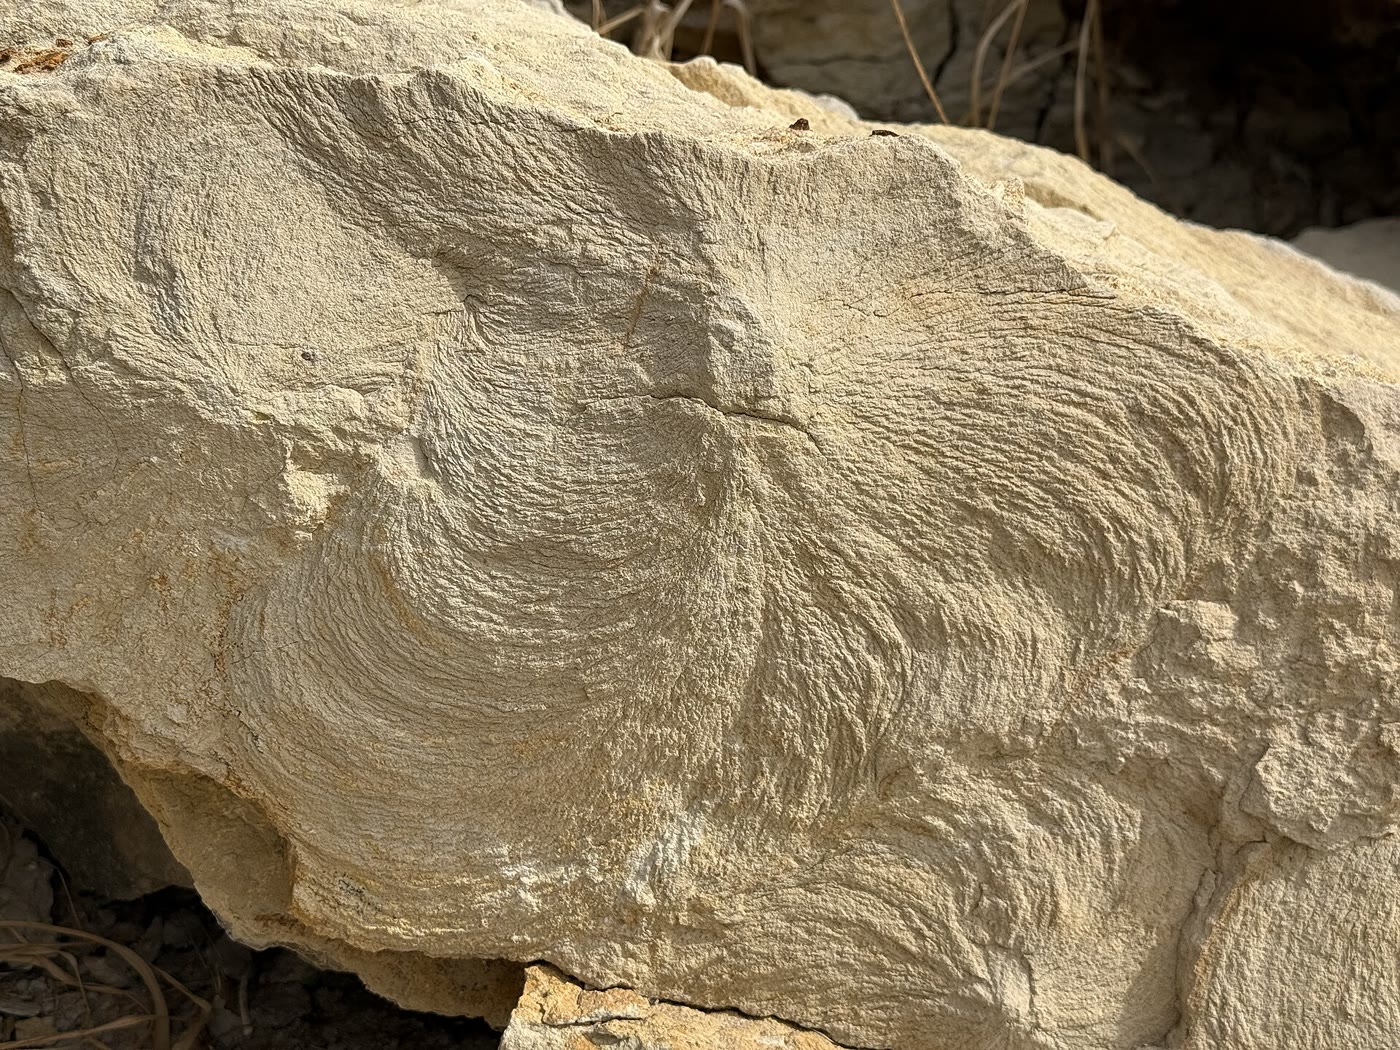
\includegraphics[width=0.5\linewidth]{images/book4/b2-20-zoophycos.jpg}
\par\smallskip{\small 葡萄牙萨格雷斯一块岩石中的 \emph{Zoophycos}：弧形条纹是
再搬运沉积物构成的螺旋状薄片的纹层。（Amada44，CC~BY~4.0，经由维基共享资源。）}
\end{omfigure}
% ledger: zhang15:zoophycos

\section{读解一片消失的海}\label{sec:b2:palaeoenvironments:varden}

各种环境彼此并列：有海滩，有近海海底，还有更深的陆架。海面上升或
海底下沉时，每种环境都会向陆地方向迁移，覆盖在邻近环境之上，
其沉积物也随之叠压于邻居的沉积物之上。连续无间断的相序垂直排列，因而
重现彼此相邻的环境次序；本科三年级分册将此规则，
即沃尔瑟定律，作为其出发点。自下而上读取的剖面，犹如海岸
在某一地点移动的影片。

瓦尔登丘陵是本丛书虚构的地区，其盖层可作为一个完整的例子。它的
厚度取自该地区的模型；下图中的化石为虚构，
但每一种都选自真实岩石中可能出现的类型。石灰岩定为托阿尔阶，
年代为 184.2 至 \qty{174.7}{Ma}；页岩则定为阿林阶至卡洛维阶，年代为
\qty{174.7}{Ma} 至 \qty{161.5}{Ma}。
% ledger: data:b4-palaeoenv, ics4:jurassic-stages

\begin{omfigure}
\centering
% figdata/bachelor-2/palaeoenv.py part log (thicknesses from figdata/shared/region.py)
\begin{tikzpicture}[x=1cm, y=0.0165cm, font=\scriptsize]
% scale
\draw[black!70] (-0.35,0) -- (-0.35,460);
\foreach \z in {0,100,...,400} {\draw[black!70] (-0.45,\z) -- (-0.35,\z) node[left=3pt] {\z};}
\node[rotate=90, anchor=south] at (-1.15,230) {盖层底面以上高度（m）};
% units
\fill[lith sandstone] (0,0) rectangle (2.2,120);
\fill[lith limestone] (0,120) rectangle (2.0,180);
\fill[lith limestone] (0,180) rectangle (1.6,300);
\fill[lith shale] (0,300) rectangle (1.1,400);
\fill[om lith={icsCretaceous!35}{om limestone}] (0,400) -- (1.4,400) -- (1.4,452)
  .. controls (1.0,466) and (0.6,446) .. (0.3,458) -- (0,455) -- cycle;
\draw[black!70] (0,0) rectangle (2.2,120);
\draw[black!70] (0,120) rectangle (2.0,180);
\draw[black!70] (0,180) rectangle (1.6,300);
\draw[black!70] (0,300) rectangle (1.1,400);
\draw[black!70] (0,400) -- (1.4,400) -- (1.4,452) .. controls (1.0,466) and (0.6,446) ..
  (0.3,458) -- (0,455) -- cycle;
\node[anchor=west, font=\tiny] at (1.45,460) {剥蚀顶面};
% unit names
\node[anchor=west, align=left] at (2.6,60) {\textbf{砂岩}，\qty{120}{m}\\三叠纪};
\node[anchor=west, align=left] at (2.6,150) {\textbf{鲕粒灰岩}，\qty{60}{m}\\托阿尔阶};
\node[anchor=west, align=left] at (2.6,240) {\textbf{细粒灰岩}，\qty{120}{m}\\托阿尔阶};
\node[anchor=west, align=left] at (2.6,350) {\textbf{页岩}，\qty{100}{m}\\阿林–卡洛维阶};
\node[anchor=west, align=left] at (2.6,424) {\textbf{白垩}\\白垩纪};
% content
\node[anchor=west, align=left, text width=6.9cm] at (6.3,60) {冲刷底面上的交错层理河道充填；
  根迹；植物碎片；无海相化石};
\node[anchor=west, align=left, text width=6.9cm] at (6.3,150) {交错层理鲕粒；竖直管状
  与 U 形潜穴；磨损的贝壳碎片};
\node[anchor=west, align=left, text width=6.9cm] at (6.3,240) {海百合骨片、腕足类、
  箭石、菊石；爬行迹与摄食潜穴；破碎贝壳层，
  底面锐利};
\node[anchor=west, align=left, text width=6.9cm] at (6.3,350) {深灰色，局部具纹层；
  黄铁矿；菊石与薄壳双壳类；浅色层中的螺旋状潜穴};
\node[anchor=west, align=left, text width=6.9cm] at (6.3,424) {球石；海胆、海绵；
  燧石结核；全层受潜穴扰动};
\foreach \z in {120,180,300,400} {\draw[black!25] (2.25,\z) -- (13.2,\z);}
\node[font=\scriptsize\bfseries, anchor=south west] at (2.6,462) {单元与年代};
\node[font=\scriptsize\bfseries, anchor=south west] at (6.3,462) {地层所含内容};
\end{tikzpicture}
\par\smallskip{\small 瓦尔登丘陵盖层的柱状图，列出各单元所含内容。
厚度取自该地区的模型，但白垩的剥蚀顶面在此截短，
（在\cref{ex:b2:palaeoenvironments:shale}的向斜中厚 \qty{766}{m}）；柱状图的宽度随粒度增大而增加；
化石及其年代均为该地区虚构。}
\end{omfigure}
% ledger: data:b4-palaeoenv, ics4:jurassic-stages

\begin{example}[瓦尔登盖层的底部]\label{ex:b2:palaeoenvironments:base}
砂岩中有冲刷底面上的河道充填、根迹与植物碎片，而无海相
化石：它是河流在陆地上沉积形成的。其上的鲕粒灰岩具有交错层理鲕粒，
（鲕粒在动荡水体中边滚动边生长），另有 Skolithos
\omterm{def:b2:palaeoenvironments:ichnofacies}{遗迹相}的竖直管状与 U 形潜穴，以及磨损的贝壳碎片，均为\omterm{def:b2:alpine-orogen:nappes}{外来的}，是滨面上的一处浅滩，
受波浪冲刷。两者之间海水侵入，该接触面记录了一次\omterm{def:b2:phanerozoic-earth:transgression}{海侵}。按
沃尔瑟定律的次序，河流平原之后是海岸，再之后是浅滩。
\end{example}
% ledger: buatois20:ichnofacies

\subsection*{海底沉积填满得有多快？}

生物带给出时长，剖面给出厚度，二者之比即为速率。但
自沉积物形成以来，其厚度已经减小：孔隙中的水已被挤出，
只有颗粒本身得以保存。

\begin{proposition}[压实地层的堆积速率]\label{prop:b2:palaeoenvironments:rate}
设厚度为 $h$、平均孔隙度为 $\varphi$ 的地层，在时长 $\Delta t$ 内，
以孔隙度 $\varphi_0$ 沉积形成，则其堆积速率为
\[
  r = \frac{h\,(1 - \varphi)}{(1 - \varphi_0)\,\Delta t}
\]
新鲜沉积物的速率，颗粒的速率则为 $h(1-\varphi)/\Delta t$，
它与 $\varphi_0$ 无关。
\end{proposition}

\begin{proof}
单位面积上，地层所含颗粒的体积为 $h(1 - \varphi)$，
即本科一年级分册所称的固体厚度。压实只排出水分，既不增加也不减少颗粒，故孔隙度为
$\varphi_0$ 的新鲜沉积物厚度为 $h_0$，满足 $h_0(1 - \varphi_0) = h(1 -
\varphi)$。以 $h_0$ 与固体厚度除以 $\Delta t$，即得两个速率。
\end{proof}

若未测得孔隙度，可由阿西定律根据深度求得。下图给出
四种岩性的该定律，以及因子 $(1 - \varphi(z))/(1 - \varphi_0)$，
即现位于深度 $z$ 的薄层须拉伸的倍数，以得到其地表厚度。
白垩与页岩初始含水量高、失水迅速：深度 \qty{1000}{m} 处的薄页岩层，
沉积时的厚度为现今的 1.68 倍，白垩层则为 2.19 倍。
% ledger: pybacktrack:compaction, pybacktrack4:limestone, data:b4-palaeoenv

\begin{omfigure}
\centering
% figdata/bachelor-2/palaeoenv.py parts poro and ratio
\begin{tikzpicture}
\begin{groupplot}[group style={group size=2 by 1, horizontal sep=1.6cm},
  width=0.46\linewidth, height=6.2cm, y dir=reverse, ymin=0, ymax=3000,
  tick label style={font=\scriptsize}, label style={font=\small}, xtick pos=bottom,
  ytick pos=left, scaled y ticks=false, yticklabel style={/pgf/number format/1000 sep={\,}}]
\nextgroupplot[xmin=0, xmax=0.75, xlabel={孔隙度 $\varphi$}, ylabel={深度 $z$ (\unit{m})},
  legend style={at={(0.5,1.04)}, anchor=south, draw=none, font=\scriptsize, legend columns=2}]
\addplot[omThm, line width=1pt] table[x=shale, y=z_m] {figdata/out/bachelor-2-palaeoenv-poro.dat};
\addlegendentry{页岩}
\addplot[omSea!80!black, line width=1pt, dashed] table[x=sandstone, y=z_m] {figdata/out/bachelor-2-palaeoenv-poro.dat};
\addlegendentry{砂岩}
\addplot[black, line width=1pt, dotted] table[x=chalk, y=z_m] {figdata/out/bachelor-2-palaeoenv-poro.dat};
\addlegendentry{白垩}
\addplot[green!45!black, line width=1pt, dash dot] table[x=limestone, y=z_m] {figdata/out/bachelor-2-palaeoenv-poro.dat};
\addlegendentry{石灰岩}
\nextgroupplot[xmin=1, xmax=3.2, xlabel={恢复因子 $(1-\varphi)/(1-\varphi_0)$}]
\addplot[omThm, line width=1pt] table[x=shale, y=z_m] {figdata/out/bachelor-2-palaeoenv-ratio.dat};
\addplot[omSea!80!black, line width=1pt, dashed] table[x=sandstone, y=z_m] {figdata/out/bachelor-2-palaeoenv-ratio.dat};
\addplot[black, line width=1pt, dotted] table[x=chalk, y=z_m] {figdata/out/bachelor-2-palaeoenv-ratio.dat};
\addplot[green!45!black, line width=1pt, dash dot] table[x=limestone, y=z_m] {figdata/out/bachelor-2-palaeoenv-ratio.dat};
\end{groupplot}
\end{tikzpicture}
\par\smallskip{\small 左图：据阿西定律得到的孔隙度随深度的变化，其中页岩、砂岩和白垩的常数取自斯卡特与
克里斯蒂（1980），石灰岩的常数取自图尔与梅纳德（2003），二者均按
pyBacktrack 中的列表。右图为现位于深度 $z$ 的薄层
恢复到地表厚度所乘的因子。}
\end{omfigure}
% ledger: pybacktrack:compaction, pybacktrack4:limestone, data:b4-palaeoenv

\begin{example}[瓦尔登页岩]\label{ex:b2:palaeoenvironments:shale}
在瓦尔登丘陵的向斜中，白垩厚 \qty{766}{m}，故页岩位于
766 至 \qty{866}{m} 之间。取页岩的常数 $\varphi_0 = 0.63$ 与 $\lambda =
\qty{1960}{m}$，则本科一年级分册所称的固体厚度为 $100 - 0.63 \times 1960 \times
(e^{-766/1960} - e^{-866/1960}) = \qty{58.4}{m}$，平均孔隙度为 0.416。以相同颗粒将其恢复到地表，
该层厚 \qty{148.6}{m}。历时 \qty{13.2}{Ma}，
自阿林阶底至卡洛维阶顶，页岩按现状以 $100/13.2 =
\qty{7.6}{m}$ 每百万年，按新鲜泥质以 $148.6/13.2 = \qty{11.3}{m}$ 每
百万年，按颗粒则为 \qty{4.4}{m} 每百万年。现厚度
低估了速率约三分之一。
\end{example}
% ledger: data:b4-palaeoenv, pybacktrack:compaction, ics4:jurassic-stages

页岩或许曾埋藏得更深，其上覆白垩已被剥蚀，此时
修正量只是下限。周末问题将该命题应用于石灰岩，其孔隙度
已经实测。

\section*{练习}\label{sec:b2:palaeoenvironments:exercises}

除非另有说明，练习所用数据如下：阿西定律 $\varphi = \varphi_0 e^{-z/\lambda}$，
其中 $\varphi_0 = 0.63$、$\lambda = \qty{1960}{m}$（页岩），$0.49$、\qty{3704}{m}（砂岩），
$0.70$、\qty{1408}{m}（白垩），$0.51$、\qty{4545}{m}（石灰岩）；方解石 \qty{2710}{kg.m^{-3}}，
孔隙水 \qty{1000}{kg.m^{-3}}；国际年代表中的各阶年龄：托阿尔阶自 184.2 至
\qty{174.7}{Ma}。
% ledger: pybacktrack:compaction, pybacktrack4:limestone, ics4:jurassic-stages

\begin{exercise}[$\star$]\label{exo:b2:palaeoenvironments:1}
在海岸海底的 51 个站点中，发现活的无脊椎动物 135 个物种，死亡的
贝壳与骨骼中有 150 个物种，另有 112 个物种也有化石记录。
(a) 将第三个数分别表示为前两个数的分数。(b) 死亡的物种数为何能超过活的？(c)
你预计哪些取食类群在\omterm{def:b2:palaeoenvironments:assemblages}{死亡组合}中代表性不足？原因何在？
\end{exercise}
% ledger: tyler25:live-dead, tyler25:soft-bodied

\begin{exercise}[$\star$]\label{exo:b2:palaeoenvironments:2}
一个晚侏罗世菊石层位平均持续 \qty{165}{ka}。(a) 五个层位共持续多久？
与 \emph{Archaeopteryx} 所给的 0.7 至 1 百万年相比较。(b) 托阿尔阶最早的
生物带自 183.73 至 \qty{182.77}{Ma}，按平均时长可容纳多少个层位？
(c) 为何追踪一个谱系的演化时，层位比生物带更为重要？
\end{exercise}
% ledger: rauhut18:archaeopteryx, alsuwaidi22:toarcian

\begin{exercise}[$\star$]\label{exo:b2:palaeoenvironments:3}
说出每组遗迹组合所属的\omterm{def:b2:palaeoenvironments:ichnofacies}{遗迹相}及沉积环境。(a) 蜿蜒的放牧迹与规则的
潜穴网，见于薄层浊积岩的底面。(b) 密集排列的直立管，见于干净的
交错层理砂岩中。(c) 大量食沉积物者形成的水平潜穴与放牧迹，见于粉砂质
层中，位于风暴砂层之间。(d) 螺旋状蹼状潜穴，见于细粒、暗色
泥中，且无波痕，产于中生代岩石。
\end{exercise}
% ledger: buatois20:ichnofacies, paz23:nereites

\begin{exercise}[$\star$]\label{exo:b2:palaeoenvironments:4}
A 层含海百合、腕足动物、珊瑚与三叶虫；同时代的 B 层含植物碎屑、
鱼骨、少量双壳类与腹足类，以及大量个体，它们只属于两个
介形虫物种。(a) 两层各自反映了怎样的水体盐度？(b) B 层缺少 A 层的各类群，
这种缺失为何可作论据，而一层中缺少一种化石则不能？
(c) 还需哪些其他观察，才能检验对 B 层的解释？
\end{exercise}
% ledger: mcgairy21:stenohaline, saleh22:echinoderms

\begin{exercise}[$\star\star$]\label{exo:b2:palaeoenvironments:5}
利用 \cref{prop:b2:palaeoenvironments:burial}，取
\cref{ex:b2:palaeoenvironments:shell} 中的贝壳，$k = \qty{0.05}{\text{年}^{-1}}$ 和 $h = \qty{0.1}{m}$。(a)
求贝壳恰有一半到达安全处时的沉积速率。(b) 速率由该值减半时，$P$
变为原来的多少倍？(c) 壳厚为两倍的贝壳，在海底
存活时间也为两倍。在 \qty{1}{mm.\text{年}^{-1}} 下，它被保存的可能性高出多少？(d) 这对
化石组合中薄壳与厚壳的比例意味着什么？
\end{exercise}
% ledger: tyler25:soft-bodied

\begin{exercise}[$\star\star$]\label{exo:b2:palaeoenvironments:6}
火山灰层测定 Chacay Melehue 处托阿尔阶底界的年龄为 $183.73$，$+0.35$，\qty{-0.50}{Ma}；
国际年代表给出 \qty{184.2}{Ma}。(a) 年代表的数值是否在不确定度范围之内？
它超出上限多少？(b) 最早的托阿尔阶生物带终止于
\qty{182.77}{Ma}，求其时长。(c) 设该带在某剖面中厚 \qty{6}{m}，
其堆积速率为多少？(d) 为何生物带在时间上处处相同，而
其厚度却因地而异？
\end{exercise}
% ledger: alsuwaidi22:toarcian, ics4:jurassic-stages

\begin{exercise}[$\star\star$]\label{exo:b2:palaeoenvironments:7}
瓦尔登向斜中，砂岩位于地面以下 1046 至 \qty{1166}{m} 之间。(a)
用阿西定律求顶部与底部的孔隙度，并由二者平均求得平均孔隙度（保留
三位小数）。(b) 求其固体厚度。(c) 用薄层因子在平均孔隙度下将其还原至
地表。(d) 精确还原给出
\qty{147.0}{m}。为何薄层估算值略偏大？
\end{exercise}
% ledger: data:b4-palaeoenv, pybacktrack:compaction

\begin{exercise}[$\star\star$]\label{exo:b2:palaeoenvironments:8}
瓦尔登石灰岩的密度测井读数为 \qty{2573}{kg.m^{-3}}，由方解石颗粒构成，孔隙中
充有水。(a) 证明孔隙度为 $\varphi = (\rho_{\text{颗粒}} -
\rho)/(\rho_{\text{颗粒}} - \rho_{\text{水}})$，并算出其值。(b) 在向斜石灰岩的中部
深度 \qty{956}{m} 处，取石灰岩常数，阿西定律预测的结果如何？
(c) 哪一种成岩作用可以解释这一差异？
\end{exercise}
% ledger: pybacktrack4:limestone, data:b4-palaeoenv

\begin{exercise}[$\star\star$]\label{exo:b2:palaeoenvironments:9}
一段由侏罗纪岩层构成的悬崖，自下而上显示：薄层浊积岩，具规则曲流与
潜穴网络；暗色泥，具螺旋状回填层潜穴；粉砂层，含食沉积物者潜穴，夹于
风暴砂之间；干净的交错层理砂，具
竖直管状潜穴；其上为含根的煤层。(a) 逐段解释。(b) 水体是加深还是
变浅？(c) 列出可能造成这一序列的两种原因，并说明
用以判别二者。(d) 从第一段直接跳到第四段、缺少中间各段，为何是一种
预警信号？
\end{exercise}
% ledger: buatois20:ichnofacies, paz23:nereites

\begin{exercise}[$\star\star\star$]\label{exo:b2:palaeoenvironments:10}
一只软体动物在海底平均可存活一年（$k = \qty{1}{\text{年}^{-1}}$），
一个贝壳可存活一世纪；二者在 $h = \qty{0.1}{m}$ 下均安全。(a) 比较二者的
在 1、10 与 \qty{100}{mm.\text{年}^{-1}} 下的保存概率。(b) 求每百个软体个体中
约有一个被保存下来的速率。(c) 此速率在持续数月的情形下是否合理？何种沉积
能更快地掩埋海底？(d) \cref{prop:b2:palaeoenvironments:burial} 的哪条假设对此类
沉积不再成立，此时公式表现如何？
\end{exercise}

\begin{exercise}[$\star\star\star$]\label{exo:b2:palaeoenvironments:11}
(a) 证明薄层因子 $(1 - \varphi(z))/(1 - \varphi_0)$ 可由
\cref{prop:b2:palaeoenvironments:rate} 导出。(b) 在瓦尔登页岩的中部深度
\qty{816}{m} 处应用之，以还原 \qty{100}{m} 页岩。(c) 与
\cref{ex:b2:palaeoenvironments:shale} 中精确的 \qty{148.6}{m} 比较，并解释差值的符号。(d) 证明
颗粒的速率不同于新沉积的速率，它可以在页岩与石灰岩之间
直接比较，而无需知道二者沉积时各自的孔隙度。
\end{exercise}
% ledger: data:b4-palaeoenv, pybacktrack:compaction

\begin{exercise}[$\star\star\star$]\label{exo:b2:palaeoenvironments:12}
设托阿尔阶菊石层平均持续 \qty{165}{ka}，与晚侏罗世的菊石层相同。
(a) 瓦尔登石灰岩的 \qty{180}{m} 中会含多少个菊石层？(b) 一个菊石层
今天代表多厚的石灰岩，以及新沉积物的厚度为多少，已知该层沉积时
厚 \qty{338}{m}？(c) 为确保找到每一个菊石层，地质学家
取样间距不超过现今厚度的一半：该间距为多少，需取多少
个样品？(d) 即便如此，为何仍可能缺失部分菊石层？
\end{exercise}
% ledger: rauhut18:archaeopteryx, ics4:jurassic-stages, data:b4-palaeoenv

\begin{problem}[{周末问题——瓦尔登丘陵的侏罗纪海}]\label{pb:b2:palaeoenvironments:1}
本题解读瓦尔登盖层的沉积环境与历史，并利用
\cref{sec:b2:palaeoenvironments:varden} 的柱状图与各练习的数据。盖层在褶皱的翼上
倾角为 \ang{12}；在向斜中，它被一口水井钻穿。

\medskip\noindent\textbf{第一部分——岩石与厚度。}
\begin{enumerate}
  \item 在翼部平坦的地面上，石灰岩出露宽度为 \qty{866}{m}，沿
        垂直走向量取。求其真厚度。
  \item 页岩出露宽度为 \qty{481}{m}。求其厚度。
  \item 哪一岩层最老？依据何种原理？
  \item 井中，页岩始于地面以下 \qty{766}{m}，石灰岩始于 \qty{866}{m}，砂岩
        始于 \qty{1046}{m}。核对各层厚度。
  \item 白垩层被地表截断。白垩纪\omterm{def:b2:phanerozoic-earth:transgression}{海退}去时，
        其厚度可作何判断？
  \item 求井中白垩层在地表处与其底部的孔隙度。
\end{enumerate}

\medskip\noindent\textbf{第二部分——沉积环境。}
\begin{enumerate}[resume]
  \item 细粒石灰岩中的海百合、腕足类、箭石与菊石，说明了
        其水体的何种特征？
  \item 其遗迹形成了哪种\omterm{def:b2:palaeoenvironments:ichnofacies}{遗迹相}？位于剖面的哪一部分？
  \item 其具尖锐底面的碎壳层记录了什么？
  \item 页岩呈暗色，局部具层理，含黄铁矿而潜穴稀少。这说明
        底层水的情况如何？
  \item 其浅色层中含螺旋状回填层潜穴。属于哪种\omterm{def:b2:palaeoenvironments:ichnofacies}{遗迹相}，对应何种环境？
  \item 页岩中的菊石是否属于海底的\omterm{def:b2:palaeoenvironments:assemblages}{生活组合}？请说明。
\end{enumerate}

\medskip\noindent\textbf{第三部分——时间与速率。}最下部的石灰岩层含有
托阿尔阶最早生物带的菊石，最上部者为最晚生物带的菊石，页岩则始于
阿林阶最早的生物带。
\begin{enumerate}[resume]
  \item 石灰岩堆积用了多长时间？
  \item 按石灰岩现今的厚度，其堆积速率为多少？
  \item 井中密度测井在石灰岩中读数为 \qty{2573}{kg.m^{-3}}。求其
        孔隙度。
  \item 灰泥沉积时的孔隙度为 0.51。求新沉积物的厚度。
  \item 求新沉积物的速率。
  \item 求颗粒的速率。
  \item 与 \cref{ex:b2:palaeoenvironments:shale} 中的页岩相比较。速率的变化
        说明碳酸盐的供应有何不同？
\end{enumerate}

\medskip\noindent\textbf{第四部分——瓦尔登上方的海。}
\begin{enumerate}[resume]
  \item 自砂岩至白垩读取柱状图，海是前进还是后退？
  \item 据 Haq 等人的长期曲线，全球海平面在约 41、57 与
        \qty{86}{m} 高于今日，对应 184、174 与 \qty{162}{Ma}。
        求石灰岩沉积期间、页岩沉积期间以及总计上升了多少？
  \item 设海底水深由浅滩处的 \qty{5}{m} 增至
        页岩顶部的 \qty{60}{m}。求自石灰岩底部至
        页岩顶部所产生的可容纳空间，计入两层的新沉积厚度，并求其平均速率。
  \item 全球海平面上升能解释其中多大份额？其余部分由何造成？
  \item 综上，瓦尔登石灰岩的灰泥在沉积时，
        以何种速率堆积而成？
\end{enumerate}
\end{problem}
% ledger: data:b4-palaeoenv, ics4:jurassic-stages, pybacktrack4:limestone, pybacktrack:compaction, data:b4-sealevel, haq87:charts, buatois20:ichnofacies, mcgairy21:stenohaline
